\documentclass[11pt]{article}
\usepackage[spanish]{babel}
\usepackage[utf8]{inputenc}
\usepackage{graphicx}
\usepackage{float}
\usepackage{url}
%Gummi|065|=)
\title{\textbf{Guía del usuario de Marvin}}
\author{Juan Heguiabehere}
\date{}
\begin{document}

\maketitle
\section{Who, Why, What, When (Introducción)}
Marvin es una plataforma para análisis y seguimiento de aplicaciones sobre la plataforma Android. Permite levantar aplicaciones desde el Google Play Store o desde archivos \texttt{.apk}, los analiza estática y dinámicamente, y lleva un registro de las diferentes versiones en una instancia de GitLab. Los componentes principales de Marvin son:
\begin{itemize}
\item \texttt{marvin-frontend}: se ocupa de la interfaz de usuario, la decompilación de aplicaciones, la base de datos y la interacción con \texttt{marvin-static-analyzer}
\item \texttt{marvin-static-analyzer}: se ocupa de buscar tipos específicos de vulnerabilidades en una aplicación. 
\item \texttt{marvin-dynamic-analyzer}: se ocupa de verificar si las vulnerabilidades encontradas estáticamente por \texttt{marvin-static-analyzer} se pueden disparar.
\end{itemize}
En principio \texttt{marvin-static-analyzer} y \texttt{marvin-dynamic-analyzer} funcionan sin interacción con el usuario, así que esta es mayormente una guía de uso de \texttt{marvin-frontend}.
\paragraph{} Marvin fue desarrollado por Juan Heguiabehere y Joaquın Rinaudo del equipo STIC de la Fundación Manuel Sadosky: \url{http://www.fundacionsadosky.
org.ar/programas/seguridad-en-tic/}.
\section{Pantalla principal}
\begin{figure}[H]
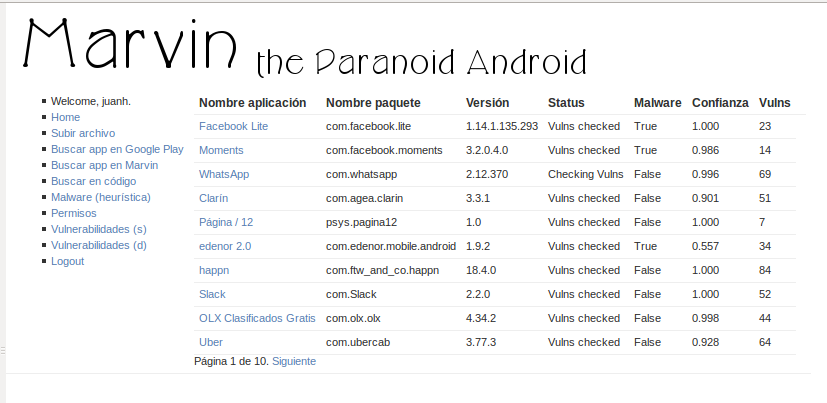
\includegraphics[width=\textwidth]{graphics/marvin_main.png}
\caption{Pantalla de inicio de Marvin}
\end{figure}
La pantalla principal de Marvin se divide en dos partes: a la izquierda está el menú de acciones y a la derecha la lista de aplicaciones. En esta lista podemos ver las últimas 10 aplicaciones subidas, con algo de información sobre las mismas. De izquierda a derecha, podemos ver:
\begin{itemize}
\item El nombre ``de fantasía'' de la aplicación.
\item El nombre de paquete de la aplicación, con el que la identifica Google Play Store.
\item El número de versión de la aplicación.
\item El estado de proceso de la aplicación (puede estar encolada, en chequeo de vulnerabilidades o ya chequeada)
\item Si la heurística de permisos determinó que la aplicación podía o no ser malware y con cuánta confianza
\item La cantidad de potenciales vulnerabilidades encontradas para la aplicación.
\end{itemize}
Clickear en el nombre de la aplicación nos lleva a su página de información (ver Sección \ref{appinfo})
\section{Menú de acciones}
\begin{figure}[H]
\begin{center}
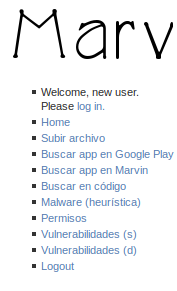
\includegraphics[width=.4\textwidth]{graphics/marvin_panel.png}
\caption{Menú de acciones}
\end{center}
\end{figure}
El menú de acciones es desde donde se disparan todas las actividades de Marvin. De arriba hacia abajo, estas son: 
\begin{itemize}
\item Ingresar (algunas acciones requieren identificarse como usuario)
\item Ir a la pantalla de inicio
\item Subir un archivo: Permite subir un archivo \texttt{.apk} que uno tenga.
\item Buscar app en Google Play: Permite descargar aplicaciones desde Google Play Store.
\item Buscar app en Marvin: Permite buscar una aplicación en Marvin, por nombre de aplicación o de paquete.
\item Buscar en código: Permite hacer búsquedas por texto en el código fuente de las aplicaciones.
\item Malware (heurística): Da una lista de las aplicaciones que el método heurístico calificó como posible malware, ordenados por la confianza en el resultado.
\item Permisos: Da una lista de los permisos encontrados por Marvin, junto con la cantidad de aplicaciones que los solicitan.
\item Vulnerabilidades(s): Da una lista de las vulnerabilidades que busca estáticamente Marvin, ordenadas por cantidad de instancias encontradas.
\item Vulnerabilidades(d): Da una lista de las vulnerabilidades que busca dinámicamente Marvin, ordenadas por cantidad de instancias encontradas.
\item Logout (desconectarse)
\end{itemize}
\subsection{Información de las aplicaciones}\label{appinfo}
En cualquier lista de aplicaciones, clickear en el nombre de la aplicación nos lleva a la pantalla de información de aplicaciones. Esta pantalla tiene tres secciones: 
\begin{itemize}
\item Metadatos y acceso a repositorios
\item Heurística y permisos
\item Componentes
\item Vulnerabilidades
\end{itemize}
\begin{figure}[H]
\begin{center}
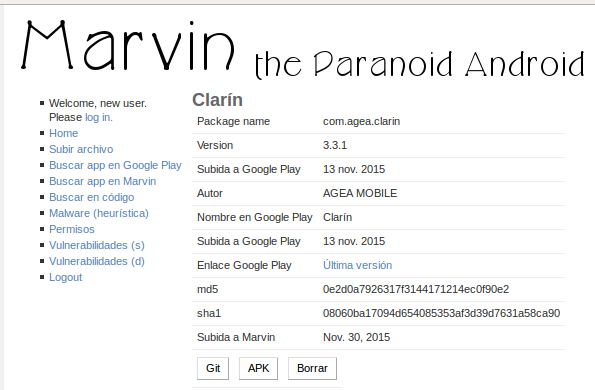
\includegraphics[width=\textwidth]{graphics/marvin_app1.png}
\caption{Metadatos y acceso a repositorios}
\end{center}
\end{figure}

En la sección de metadatos y acceso a los repositorios, podemos ver datos como la fecha de subida de una aplicación a Google Play, el número de versión o los checksums del archivo, así como acceder a los repositorios de código fuente (el botón llamado Git\footnote{Este botón permanecerá grisado hasta que los fuentes hayan terminado de cargarse en el repositorio.}), del APK propiamente dicho, o de Google Play (aunque en ese caso nos lleva a la última versión sin importar cuál estemos viendo). También nos permite borrar una aplicación de Marvin.

\begin{figure}[H]
\begin{center}
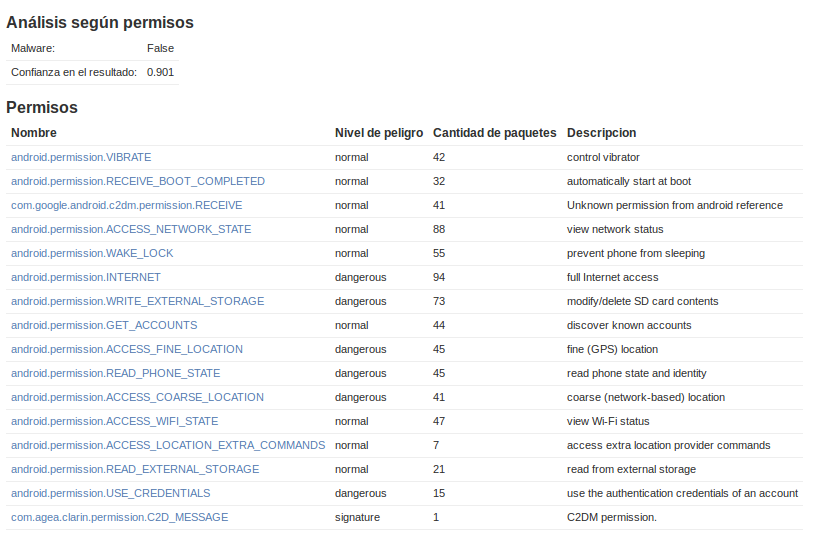
\includegraphics[width=\textwidth]{graphics/marvin_app2.png}
\caption{Heurística y permisos}
\end{center}
\end{figure}
La sección de heurística y permisos nos muestra el resultado del análisis bayesiano de permisos, y los permisos que solicita la aplicación. La lista de permisos nos muestra el nombre, el nivel de peligro del mismo, la cantidad de paquetes que lo solicitan y una descripción somera de lo que permite hacer o acceder. Clickear en el nombre de alguno de los permisos nos lleva a una página con información y estadísticas del mismo (ver Sección \ref{permisos}).
\begin{figure}[H]
\begin{center}
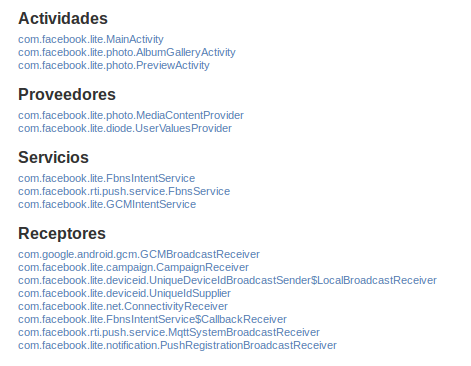
\includegraphics[width=.8\textwidth]{graphics/marvin_app3.png}
\caption{Componentes}
\end{center}
\end{figure}
 
La sección de componentes nos muestra las actividades, proveedores, servicios y receptores de una aplicación. Si se terminó de decompilar, clickear en alguno de estos items nos lleva a una nueva pestaña con el código fuente que lo implementa.
\begin{figure}[H]
\begin{center}
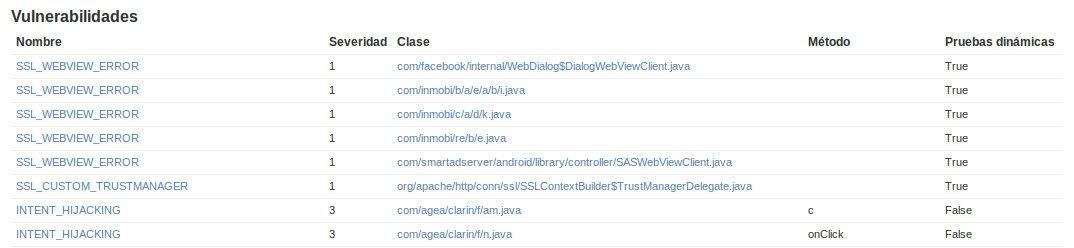
\includegraphics[width=\textwidth]{graphics/marvin_app4.png}
\caption{Vulnerabilidades}
\end{center}
\end{figure}

La sección de vulnerabilidades nos muestra una lista de las vulnerabilidades encontradas por \texttt{marvin-static-analyzer}; podemos ver el nombre de la vulnerabilidad, la severidad de la misma, la clase en que fue encontrada, el método si corresponde, y si la vulnerabilidad se puede verificar mediante análisis dinámico. Clickear en el nombre de la vulnerabilidad nos da información sobre la misma en general, mientras que clickear en el nombre de la clase nos abre una nueva pestaña con la página de GitLab correspondiente al código fuente de la misma.

\subsection{Búsqueda en Google Play Store}
Marvin puede buscar y descargar aplicaciones de Google Play. Para esto, seleccionar ``Buscar app en Google Play'' en el menú de acciones, ingresar los términos de búsqueda deseados en el campo de texto que aparece al final del menú, y presionar Enter (o el botón de Search).
\begin{figure}[H]
\begin{center}
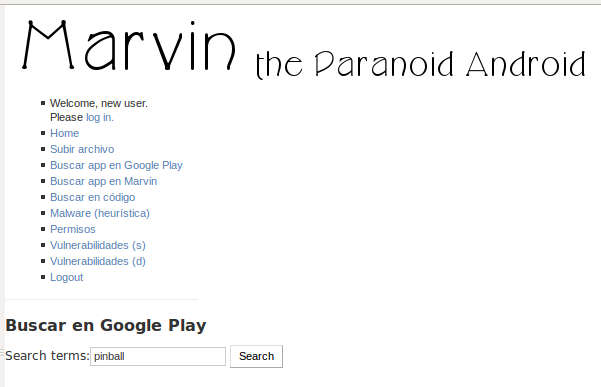
\includegraphics[width=\textwidth]{graphics/marvin_gplay.png}
\caption{Búsqueda en Google Play - Términos de búsqueda}
\end{center}
\end{figure}

La pantalla de resultados es como se ve en la Figura \ref{gplay2}: tiene algunos datos básicos de cada aplicación, más la fecha de carga en Google Play y la cantidad de descargas. Si elegimos alguna de estas aplicaciones, pasamos a una pantalla como la de la Figura \ref{gplay3}, donde se ven algunos datos más de la aplicación tales como la descripción y los permisos que solicita, y se puede solicitar la descarga de la aplicación desde Google Play Store. Esto hace que se descargue la aplicación y se procese.
El análisis: Primero la aplicación es decompilada, luego se realiza el análisis estático. Sin embargo, como el proceso de carga de los fuentes en la base de datos y el GitLab toma tiempo, usualmente el análisis termina antes de que el repositorio esté listo. Hasta que los fuentes no están terminados de subir a GitLab, los links al código fuente darán error 404.

\begin{figure}[H]
\begin{center}
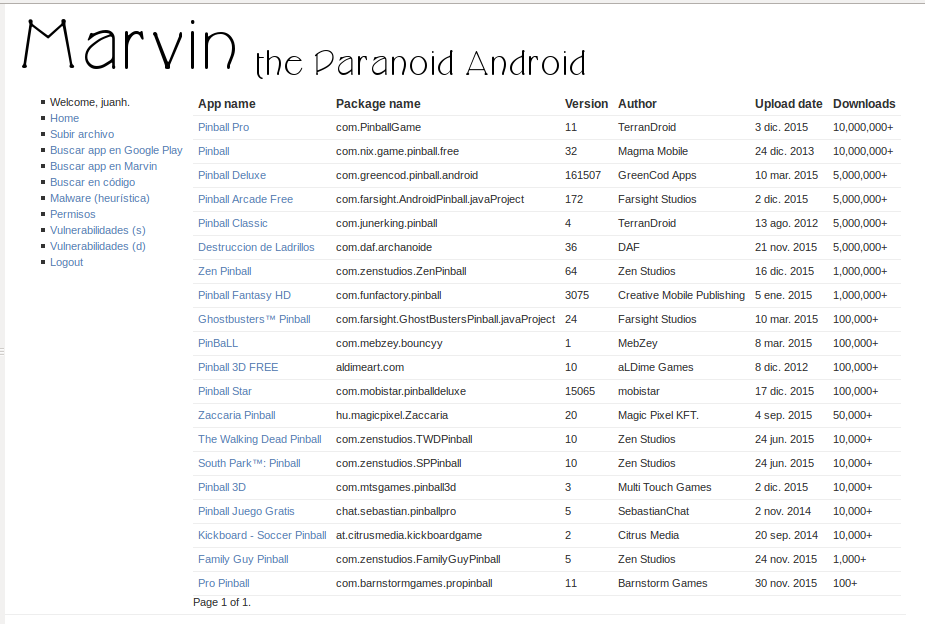
\includegraphics[width=.8\textwidth]{graphics/marvin_gplay2.png}
\caption{Búsqueda en Google Play - Resultados} \label{gplay2}
\end{center}
\end{figure}

\begin{figure}[H]
\begin{center}
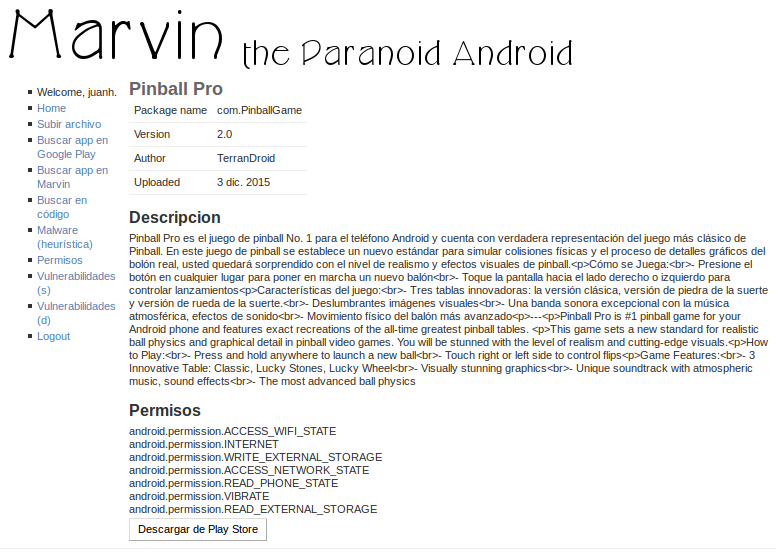
\includegraphics[width=.8\textwidth]{graphics/marvin_gplay3.png}
\caption{Búsqueda en Google Play - Descripción} \label{gplay3}
\end{center}
\end{figure}

\subsection{Buscar en código}
La opción ``Buscar en código'' nos permite buscar strings arbitrarios en la base de código de Marvin, por ejemplo para buscar casos de utilización de alguna biblioteca de Java o servicio de Android. Simplemente escribir los términos de búsqueda en el campo provisto y dar Enter, como se ve en la Figura \ref{ssource1}. Los resultados se verán como los de la Figura \ref{ssource2}: para cada coincidencia, se muestra el nombre de la clase, la aplicación a la que pertenece, y el largo del archivo fuente. Clickear en el nombre del archivo nos lleva al archivo mismo en el repositorio GitLab.
\begin{figure}[H]
\begin{center}
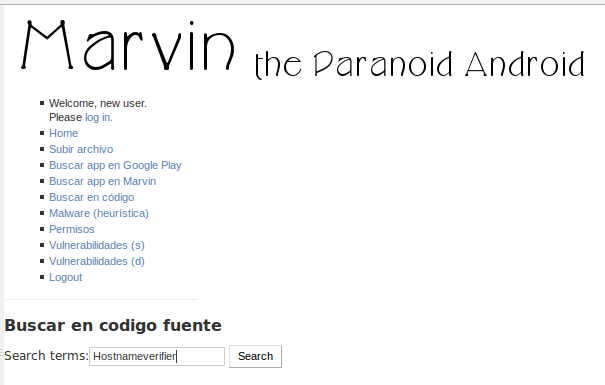
\includegraphics[width=\textwidth]{graphics/marvin_searchsource1.png}
\caption{Búsqueda en código fuente} \label{ssource1}
\end{center}
\end{figure}

\begin{figure}[H]
\begin{center}
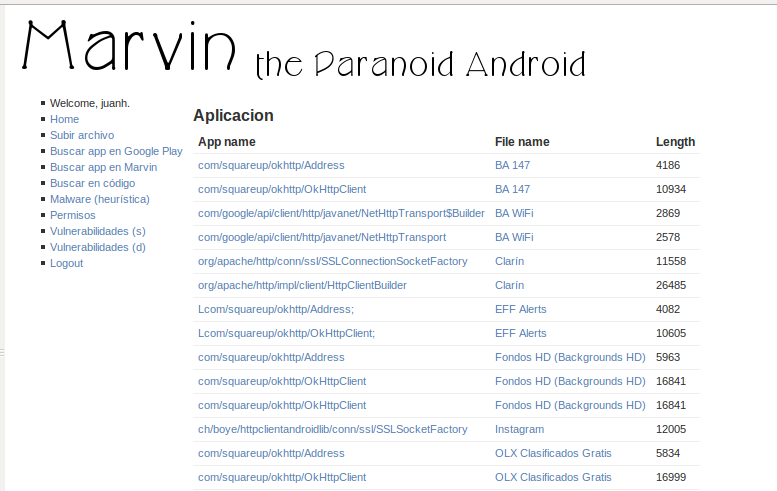
\includegraphics[width=\textwidth]{graphics/marvin_searchsource2.png}
\caption{Búsqueda en código fuente - Resultados} \label{ssource2}
\end{center}
\end{figure}

\subsection{Malware (heurística)}
En esta opción podemos ver las aplicaciones que según la heurística tienen más probabilidades de ser en realidad malware. Junto a la información de versión, se ve un indicador de la confianza que tiene Marvin en su resultado, y la cantidad de vulnerabilidades encontradas para cada aplicación.
\begin{figure}[H]
\begin{center}
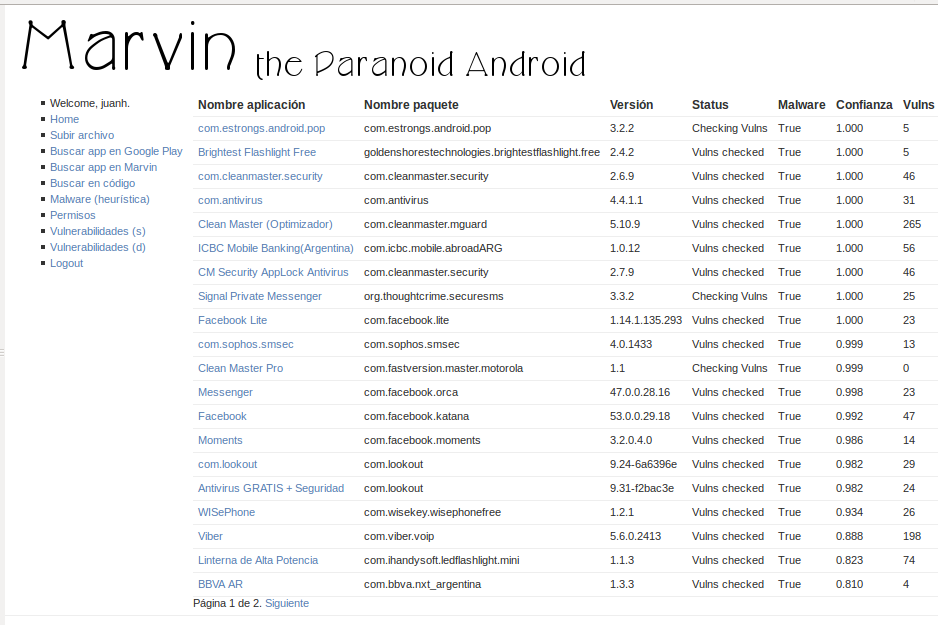
\includegraphics[width=\textwidth]{graphics/marvin_bayesboys.png}
\caption{Malware según la heurística de permisos} \label{bayes}
\end{center}
\end{figure}
\subsection{Permisos}\label{permisos}
La opción Permisos nos permite ver los permisos relevados por Marvin entre todas las aplicaciones, y para éstos una descripción, su nivel de riesgo y la cantidad de aplicaciones relevadas que lo solicitan (ver Figura \ref{perms}). Si clickeamos en el nombre de algún permiso, Marvin nos muestra las aplicaciones que lo solicitan, como se ve en la Figura \ref{appsbyperm}
\begin{figure}[H]
\begin{center}
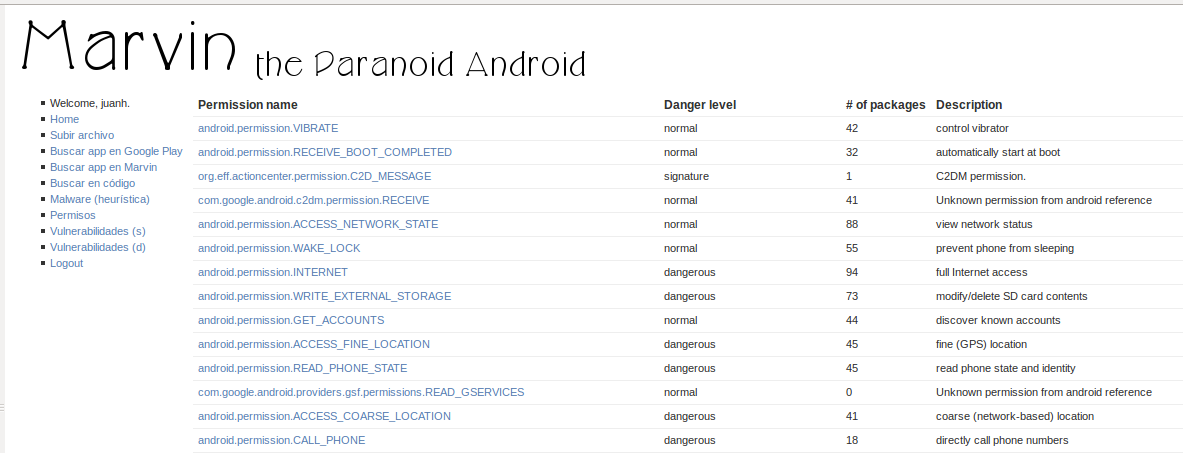
\includegraphics[width=\textwidth]{graphics/marvin_permissions.png}
\caption{Permisos relevados por Marvin} \label{perms}
\end{center}
\end{figure}

\begin{figure}[H]
\begin{center}
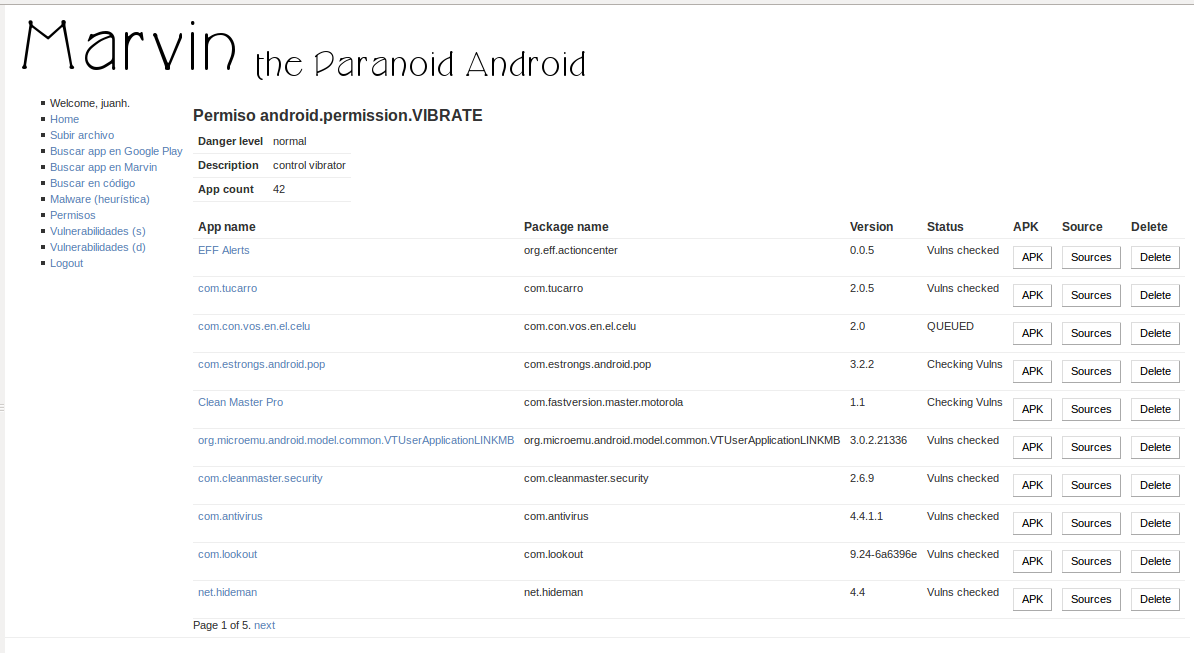
\includegraphics[width=\textwidth]{graphics/marvin_permissions2.png}
\caption{Aplicaciones que solicitan un permiso dado} \label{appsbyperm}
\end{center}
\end{figure}

\subsection{Vulnerabilidades}
En esta sección, podemos ver las vulnerabilidades que Marvin conoce y puede detectar, tanto estática como dinámicamente. Algunas de las vulnerabilidades que encuentra mediante el análisis estático pueden ser verificadas mediante análisis dinámico, y otras se buscan directamente mediante el análisis dinámico. Para cada uno de los tipos de vulnerabilidades, Marvin muestra una lista ordenada por la cantidad de aplicaciones en donde se encontró la vulnerabilidad (Ver Figura \ref{vulns}). Si clickeamos en el nombre de la vulnerabilidad, Marvin nos muestra una lista de aplicaciones en donde ésta se encontró (ver Figura \ref{vulns2}).


\begin{figure}[H]
\begin{center}
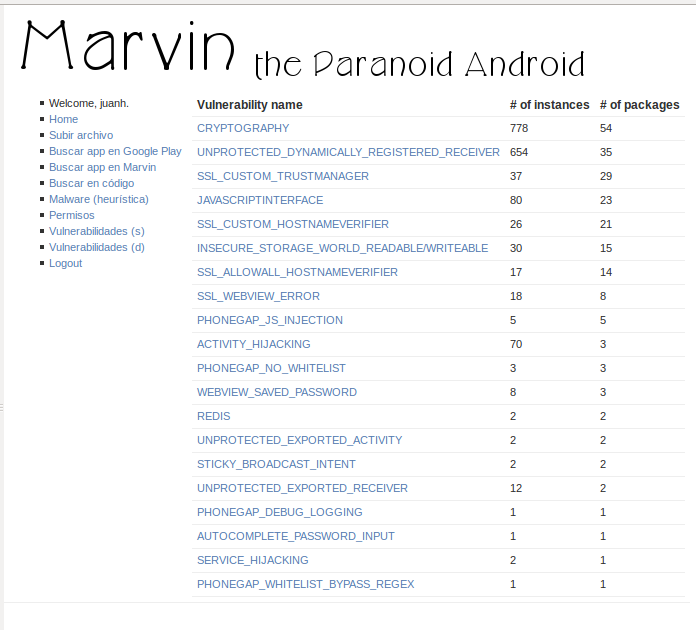
\includegraphics[width=\textwidth]{graphics/marvin_vulns.png}
\caption{Lista de vulnerabilidades conocidas por Marvin} \label{vulns}
\end{center}
\end{figure}

\begin{figure}[H]
\begin{center}
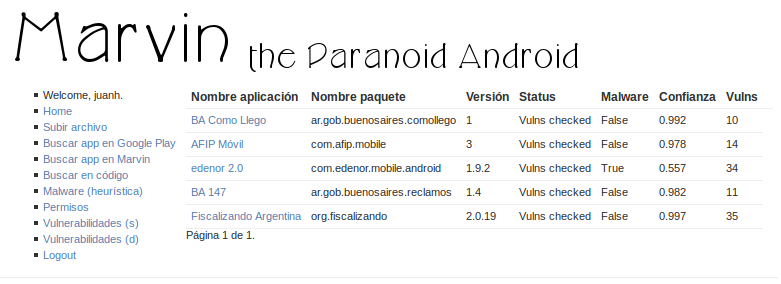
\includegraphics[width=\textwidth]{graphics/marvin_vulns2.png}
\caption{Lista de aplicaciones con una vulnerabilidad determinada} \label{vulns2}
\end{center}
\end{figure}

\section{Administración}
En la sección de Administración se manejan las cuentas de usuario de Marvin y la cuenta de acceso al Play Store. Se accede a esta sección por \texttt{http://\{url\_marvin\}/admin}.

\begin{figure}[H]
\begin{center}
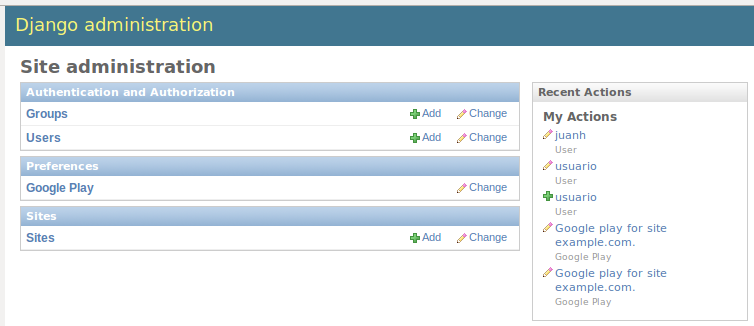
\includegraphics[width=\textwidth]{graphics/marvin1.png}
\caption{Sección de administración} \label{admin}
\end{center}
\end{figure}
\subsection{Cuentas de usuario}
Clickeando en ``Users'' ingresamos a la administración de usuarios:
\begin{figure}[H]
\begin{center}
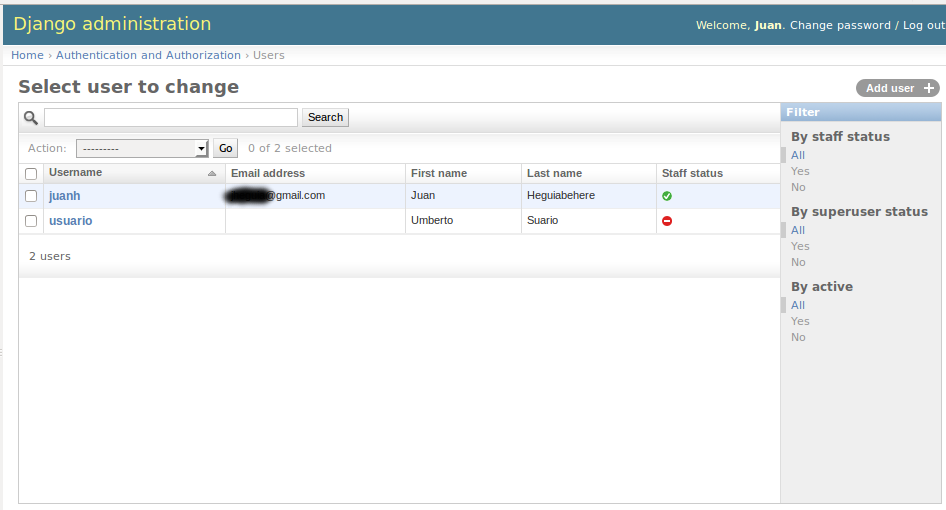
\includegraphics[width=\textwidth]{graphics/marvin2.png}
\caption{Sección de administración - Usuarios} \label{adminus}
\end{center}
\end{figure}
En esta sección se pueden dar de alta o baja cuentas, necesarias para modificar el estado de una aplicación en Marvin (léase dar de alta aplicaciones desde Google Play o archivo, borrar aplicaciones). De momento todos los usuarios no-administradores tienen permisos completos sobre todo el repositorio. 

El alta de un usuario es trivial:
\begin{figure}[H]
\begin{center}
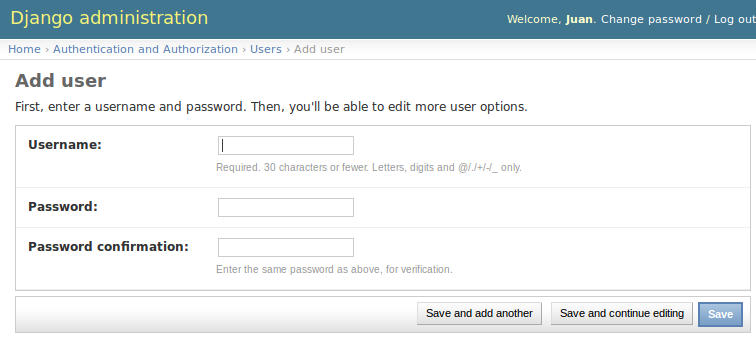
\includegraphics[width=\textwidth]{graphics/marvin4.png}
\caption{Sección de administración - Alta de usuario} \label{altaus}
\end{center}
\end{figure}
\subsection{Cuenta de Google Play}
\begin{figure}[H]
\begin{center}
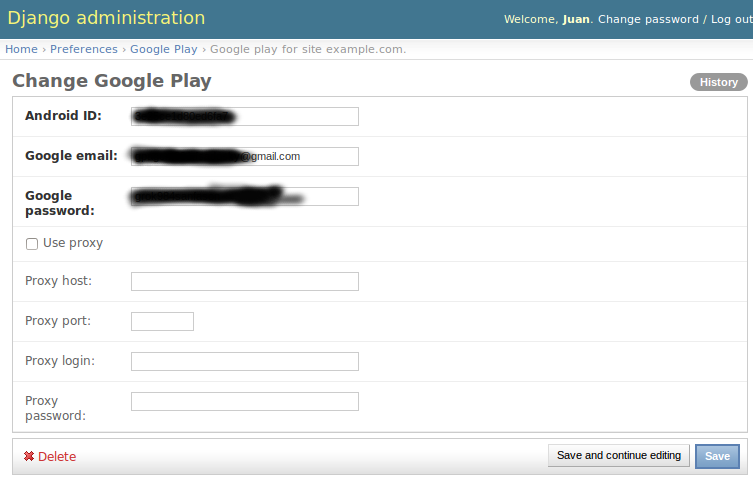
\includegraphics[width=\textwidth]{graphics/marvin3.png}
\caption{Sección de administración - Usuario Google Play} \label{googleplay_acct}
\end{center}
\end{figure}
La sección de Cuenta de Google Play nos permite ingresar los datos de una cuenta habilitada para acceder al Play Store. Para habilitar una cuenta de Google ya existente, se puede utilizar el programa \texttt{android-checkin} de Nicolas Viennot:
\texttt{https://github.com/nviennot/android-checkin}, o por supuesto haber usado esa cuenta en un teléfono Android.
\end{document}
